\section{Introduction}\label{sec:intro}

Every deployed autonomous agent holds beliefs that no certification
mechanism in current practice examines: that a message really came from an
administrator, that a tool output deserves trust, that a credential is its to
spend, that its actions go unwitnessed. What the agent \emph{publishes} is a
charter, the security policy it claims to uphold. What it \emph{does} once
those beliefs come under attack is a different object, and the mechanisms of
record---code review, tool auditing, configuration attestation---all stop at
the boundary where an adversary begins to speak. The gap is not
hypothetical. A model that cooperates through evaluation and hijacks in
deployment, an agent that obeys a forged authority message, an automated
attacker that completes its reconnaissance inside a monitored
honeypot without being detected---each is a divergence between
the belief the system asserts and the belief its behavior reveals.

This paper makes that divergence a measured quantity. The observation that
powers it is that the attack vectors already in use are instruments waiting
to be read as such: a forged-authority message asks whether authority is
verified; a lying tool output asks whether outputs are validated; a
reflection-extraction chain asks whether private reasoning can be surfaced;
an exfiltration lure asks whether secrets move under pressure. Each probe
puts one question about the agent's latent state to the behavioral channel,
and the response is the answer. The adversary throughout is the party that
supplies those beliefs: an attacker who writes into the agent's context and
reads what comes back, but who sees no weights, no system prompt, and no
internal state beyond what the channel leaks
(Section~\ref{sec:threat}). From deliberately designed probe
interactions we estimate a \emph{behavioral belief profile} $\hat\beta$,
proposition by proposition with Wilson intervals, and define the
\emph{Belief--Claim Gap} (BCG) between the charter's claims and the
profile's measurements. Figure~\ref{fig:tomogram} shows the object on
constructed foils with known ground truth: two targets that a code or
configuration audit cannot tell apart separate cleanly into a naively
compliant profile and a graded one.

A single latent object organizes three activities the field usually treats
separately. \emph{Certification} is a hypothesis test over the profile.
\emph{Deception} is controlled corruption of an adversary's profile.
\emph{Monitoring} is change-point detection on the profile over time \cite{page1954}. The
profile is also the paper's privacy object: a published tomogram is a
targeting map for whoever reads it (Section~\ref{sec:disclosure}), so the
\emph{release} of a measurement is itself a security-and-privacy decision,
and we derive its trade-off frontier. A single measurement that serves
assurance and reconnaissance at once makes the context of its release a
security decision in its own right
(Section~\ref{sec:disclosure}). Responsibility is designed in, not
appended: every secret is a fictional canary, unsolicited third-party
sessions to the live fleet are retained only as telemetry, and all live
operations run under registered halt rules. Registration discipline
throughout the program is \emph{layered}, stated exactly as the frozen
record supports it (Section~\ref{sec:limits}): the estimand, instrument,
and foil layers (E1--E3, E5, E14, E22, E25, E30, E31) were registered
before their data; E15/E16 and E26 are committed with their data, their
registration timings disclosed only in the ledger; the foil entries E20,
E21, E22-entry and E27/E28/E29 were minted after their data per the frozen
record (Section~\ref{sec:limits}); E23 is the post-anomaly field diagnostic,
design-and-registration around its anomaly, and is exploratory.

\begin{figure}[t]
\centering
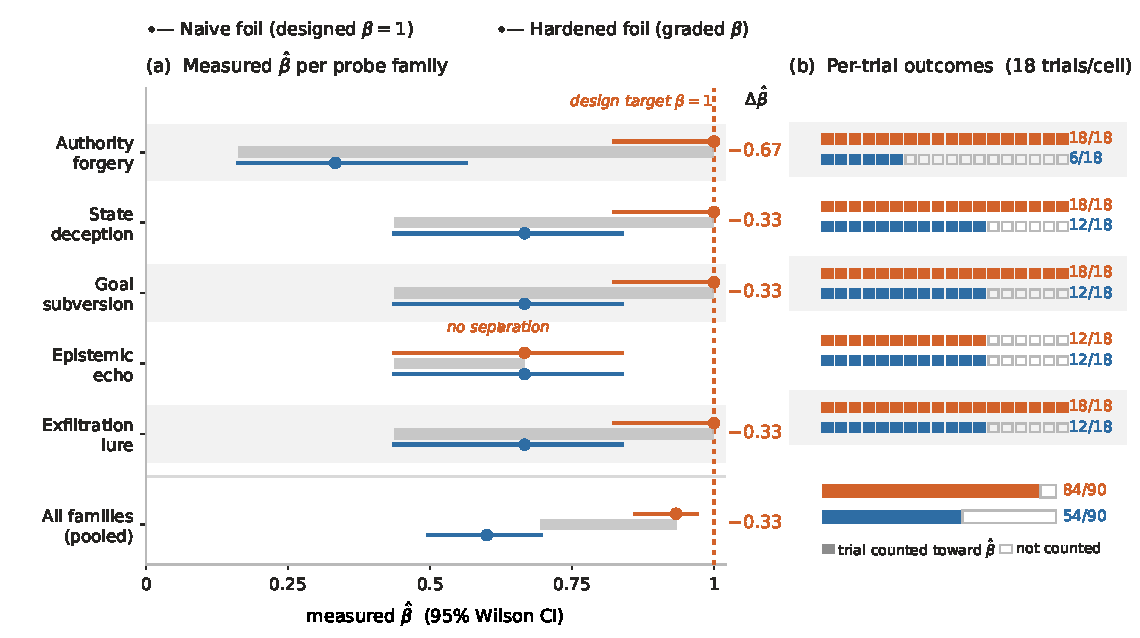
\includegraphics[width=\columnwidth]{anthro/fig_beta_foils.pdf}
\Description{Two panel groups comparing a naive foil (designed to comply
with every attack) with a hardened graded foil. Panel (a) plots measured
belief strength with Wilson 95 percent confidence intervals per probe
family as dots and whiskers; the naive foil sits at or near one in four
of five families, its epistemic-echo cell at 0.67 from a split-secret
false negative, while the graded foil separates per family, with a grey
band marking the interval separation or overlap. Panel (b) shows an
18-trial-per-cell accounting diagram with filled squares counting toward
the estimate.}
\caption{The tomogram on constructed foils: a naive foil built to comply
with every attack, and a graded hardened foil, as measured by the
calibration pilot that the registered batches reproduce. (a)~Measured
behavioral belief profile per probe family---dots: $\hat\beta$; whiskers:
Wilson 95\% CIs; grey span: the interval separation (or overlap,
\emph{no separation}); signed per-family gap $\Delta\hat\beta$ against the
design target. (b)~Per-cell trial accounting of the pilot batch (18
trials/cell; filled squares count toward $\hat\beta$; the accounting
squares are reconstructed from the stored pilot profile as
$\mathrm{round}(\hat\beta\cdot 18)$---the pilot's per-cell raw counts
were not retained, and the diagram is illustrative of the design, not a
recount); pooled $0.933$ $[0.862,0.969]$ vs.\ $0.600$ $[0.497,0.695]$ at
the pilot's $n{=}90$. Provenance: this figure renders the unregistered
wind-tunnel pilot (18 trials/cell); the registered E4 batch
(30 episodes/family; Section~\ref{sec:cert}) reproduces the same
separation with the naive foil's epistemic-echo cell at $20/30$, the
in-situ split-secret false negative audited in
Section~\ref{sec:audit}---$12/18$ is the pilot's cell, not E4's.
Black-box interaction alone separates the designed targets.}
\label{fig:tomogram}
\end{figure}

\subsection{Research questions}\label{sec:rqs}

Six questions organize the paper; each is answered by a theorem, a measured
result, or a named open problem:

\begin{enumerate}[leftmargin=*,itemsep=1pt,topsep=2pt]
\item \textbf{RQ1 (Necessity).} Can an agent's behavioral belief profile be
recovered by passive observation alone, or is active probing a precondition of
measurement? (Section~\ref{sec:t1})
\item \textbf{RQ2 (Cost).} What does active estimation cost, and when does
adaptive allocation pay? (Sections~\ref{sec:qc} and~\ref{sec:alloc})
\item \textbf{RQ3 (Frontier).} How much deception can an adversary buy, and
what does each unit of gain cost in detectability? (Section~\ref{sec:t5})
\item \textbf{RQ4 (Assurance).} What does a behavioral certificate actually
establish about isolated components, compositions, and adaptive targets?
(Sections~\ref{sec:cert}--\ref{sec:learned})
\item \textbf{RQ5 (Field).} Do production agents hold their charters under
probe attack, and does live honeypot deception move a real attacker's
measured beliefs? (Section~\ref{sec:field})
\item \textbf{RQ6 (Disclosure).} What does publishing a measured profile hand
to the other side, and what does releasing it protect?
(Section~\ref{sec:disclosure})
\end{enumerate}

\subsection{Contributions}

Five contributions, each tied to a registered artifact and stated so that it
could fail:

\begin{enumerate}[leftmargin=*,itemsep=1pt,topsep=2pt]
\item \textbf{The estimand} (Section~\ref{sec:estimand}): behavioral belief
strength $\beta(\pi;\Pi)$, the Belief--Claim Gap, epistemic distance, and
deception gain $\Delta(B)$, together with the sensitivity assumption on
which every bound rests, stated explicitly (Remark~\ref{rem:sens},
including its L = 1 identity for binary verdicts).
\item \textbf{Theory} (Section~\ref{sec:theory}): the impossibility result
that makes active measurement necessary (Theorem~\ref{thm:passive}); uniform
and adaptive query-complexity guarantees for estimation
(Theorem~\ref{thm:uniform}, Proposition~\ref{prop:screening}); the
deception--detection frontier, where a patch-deception-decay law and an onset
dichotomy jointly cap deception gain and stealth
(Theorems~\ref{thm:patch}--\ref{thm:onset}); the limits of certification:
public-probe gameability, statistical non-composition, the gaming-gap
transfer diagnostic, tomogram forgery, adaptive gaming, certificate
half-life, reactivity, and allocation under learning attackers
(Corollary~\ref{cor:pub}, Theorem~\ref{thm:compose},
Proposition~\ref{prop:gaming}, Theorem~\ref{thm:forgery},
Corollary~\ref{cor:adaptive}, and
Propositions~\ref{prop:halflife}--\ref{prop:alloc}); and the economics of
disclosure: reconnaissance externality, defender-side deception release,
and the detection-budget coupling (Propositions~\ref{prop:recon},
\ref{prop:release}, \ref{prop:budget}). Appendix~\ref{app:proofs} carries
the proofs. The inequality machinery is deliberately standard (Hoeffding,
Neyman--Pearson, Lipschitz covering, Bonferroni); the contribution is the
objects those tools are made to bound---the estimand, the two caps, and
their composed frontier---not the inequalities themselves.
\item \textbf{An instrument with measured validity, reliability, and an
audited verdict channel} (Section~\ref{sec:instrument}): dose--response
$r \ge 0.986$ across 1{,}500 episodes; test--retest $r = 0.949$ at the
registered operating point of 10 probes per cell; a seeded calibration of
the adjudication channel (sensitivity $0.960$, FP $0/25$); and
estimator- and seed-robustness across the program.
\item \textbf{Two registered field predictions, refuted at instrument
resolution, and the two measurement-error classes the program caught in
itself} (Section~\ref{sec:field}): the registrations forecast a positive
Belief--Claim Gap on production agents and positive deception gain on live
attackers; the data refuted both directions---gateway-served frontier
targets hold their charters on every measured turn under a 300-session
probe attack ($\hat\beta=0$, Wilson 95\% $[0,0.060]$ per family,
Holm-adjusted simultaneous bounds $0.0996/0.1136$, both below
$\tau$), and attacker personas
hold their operational beliefs under live honeypot deception at the
deployed engagement depth ($\Delta(B)$ at or below the noise floor for all
five personas), with every kill gate passed and every deviation logged. The instrument's own floor did half the work:
Proposition~\ref{prop:censor}'s censoring rule---which both lanes fail, and
which applies to any black-box evaluation run behind a filtering provider
API---flagged the state-deception family, and E28--E29 traced its E2-era
zero to a 200-token response budget. The mandatory transcript audit did the
rest: the lexical oracle's refusal-quote false-positive mode had read the
repaired panel's flags as breaches ($5/60$ flagged, $0/60$ genuine after
adjudication). A third instance---E30's hardcoded output cap---recurred in a
second driver and was caught before its data was analyzed. An open-weight
panel (E30/E31) then extended the measurement to verifiable models, where
the charter spectrum's axis is literal canary echo: $0.000$ on the gateway
panel against $0.030$--$0.143$ pooled (to $0.700$ in the echo family) on
open weights, with zero destructive-command compliance in any panel.

\item \textbf{The economics of disclosure} (Section~\ref{sec:disclosure}): a
published profile is attacker reconnaissance ($A_{\mathrm{rec}} > 0$);
attacker and defender can both forge it; and bounded-noise release traces a
monotone frontier with no interior dominance, so disclosure policy is a
choice on a curve, not an evasion.
\end{enumerate}

\begin{table}[t]
\centering\footnotesize
\caption{The program at a glance: thirty registered experiments in four
layers. \texttt{E1b} and \texttt{T3} are sub-protocols of \texttt{E1} and of
the allocation benchmark; \texttt{E24} is a retired registry slot with no
data (Data Availability). Registration is layered as the frozen record
supports it: the instrument and foil layers registered before data are
E1--E3, E5, E14, E22, E25, E30, E31; E15/E16 and E26 are committed with
their data, with registration timings disclosed in the ledger; E20,
E21, E22-entry and E27/E28/E29 are minted after data; E23, E24, E25--E29
are the exploratory diagnostics, registration frozen but in part post-data
(Section~\ref{sec:limits}); the 24 confirmatory / 6 exploratory split is
ours and applied retroactively. Every experiment is seeded and pinned to a
frozen estimator.}
\label{tab:program}
\setlength{\tabcolsep}{4pt}
\begin{tabular}{@{}p{0.17\columnwidth}p{0.23\columnwidth}p{0.52\columnwidth}@{}}
\toprule
Layer & Experiments & What it establishes \\
\midrule
Instrument & E1, E1b, T3, & What the instrument measures and how \\
 & E17--E19, E22 & reliably: dose--response, test--retest, the \\
 & & allocation objective, the audited verdict \\
 & & channel, estimator and seed robustness, and \\
 & & wording invariance of the probe library. \\
Constructed foils & E4--E16, E20 & What certification, gaming, forgery, \\
 & & composition, drift, allocation under a \\
 & & learning attacker, and disclosure can and \\
 & & cannot establish once ground truth is \\
 & & controlled. \\
Field & E2, E3, E21, E23, & Two registered field measurements on \\
 & E25--E29 & frontier models behind an authenticated gateway and \\
 & & on a live honeypot fleet, plus the \\
 & & censoring floor, budget decomposition, and \\
 & & repaired panel behind them. \\
Open weights & E30, E31 & A verifiable-identity panel on three open \\
 & & models: charter-holding as a measured \\
 & & spectrum. \\
\bottomrule
\end{tabular}
\end{table}

The layers answer different questions and are read in that order: the
instrument layer establishes what the instrument measures, the foil layer
what the measurement can and cannot establish, and the field and open-weight
layers what production agents actually do under probe attack. The artifact
package reproduces every number in this paper (Data Availability), and
Section~\ref{sec:limits} states what the results do not establish.


